% This must be in the first 5 lines to tell arXiv to use pdfLaTeX, which is strongly recommended.
\pdfoutput=1
% In particular, the hyperref package requires pdfLaTeX in order to break URLs across lines.

\documentclass[11pt]{article}

\usepackage[a4paper, total={6in, 8in}]{geometry}
\usepackage{lineno}
\linenumbers

\usepackage{caption,subcaption}

\usepackage{mystyle}

\usetikzlibrary{calc,patterns,angles,quotes}    
\usetikzlibrary{decorations.pathmorphing}
\tikzset{snake it/.style={decorate, decoration=snake}}

\usepackage{natbib}
\bibliographystyle{abbrvnat}
\usepackage{hyperref}

% Standard package includes
\usepackage{times}
\usepackage{latexsym}

% For proper rendering and hyphenation of words containing Latin characters (including in bib files)
\usepackage[T1]{fontenc}
% For Vietnamese characters
% \usepackage[T5]{fontenc}
% See https://www.latex-project.org/help/documentation/encguide.pdf for other character sets

% This assumes your files are encoded as UTF8
\usepackage[utf8]{inputenc}


\title{Learning to Augment: Non-Autoregressive Translation}

\author{Justin Chiu \\
  Cornell Tech \\
  \texttt{jtc257@cornell.edu}}

\begin{document}
\maketitle
\begin{abstract}
\end{abstract}

\section{Introduction}
{\color{red}High level pitch}
MLE is bad when the model is misspecified.
Outside of language (ie in non-autoregressive image and audio synthesis),
GANs have found success at training misspecified models.
Within language, GANs are plagued by unstable training (high variance grad estimators).
However, seq-KD approaches, which also serve to simplify data, have been successful.
We seek to improve upon seq-KD, which does not take into account the model we wish to train.
{\color{red}/High level pitch}

Learned models of data are often misspecified.
When the goal of modeling is not density estimation
but some alternative objective, this misspecification may lead to undesirable
behaviour under the maximum likelihood objective.
In this note, we consider learned data augmentation techniques to edit
each data point so that the augmented data is more amenable to a particular model class,
while preserving the properties we care about.

A concrete example of a setup where maximum likelihood may not be desirable is
non-autoregressive translation, which we focus on in this note.
In translation, the goal is to translate a source sentence from one language
into a sentence in a different target language.
The success of translation is measured by the BLEU score
between our generated translation and the true reference target sentence.
As the BLEU score is not a function of distributional closeness to the true data,
translation systems often discard distributional information and
output a single translation of a source sentence.
However, the training objective is still often maximum likelihood, a function of
the model distribution.

In the case of non-autoregressive translation, this results in undesirable behaviour.
As non-autoregressive models cannot model output dependencies,
resulting models trained via maximum likelihood using the true distribution
often have pathological errors due to misspecification,
and therefore poor BLEU scores.
We aim to resolve this via data augmentation.

Prior work shows that distillation is a successful data augmentation approach.
We instead rely on neural editor models \citep{edit},
which are a trainable alternative to data augmentation \citep{recombine}.

\section{Problem Setup}
Given a source sentence $x$, our goal in translation is to model the target sentence $y$.
We approach this problem with the following generative model:
\begin{itemize}
\item Given the source sentence $x$, we choose a proposal translation
    from a nonautoregressive (NAR) translation model  $\hat{y}\sim p(\hat{y} \mid x)$
\item We choose a noise vector $z \sim p(z \mid x)$ from a conditional prior
\item We choose a final translation $y \sim p(y \mid \hat{y}, z, x)$ from an edit model
\end{itemize}
This yields the joint distribution
$$p(y,\hat{y},z \mid x) = p(y \mid \hat{y}, z, x)p(\hat(y) \mid x)p(z \mid x)$$
The generative model is shown in Figure \ref{fig:gen-model}.

\begin{figure}
\centering
\begin{subfigure}{0.48\textwidth}
\centering
\begin{tikzpicture}
\node[obs]                (x)  {$x$};
\node[latent, right=of x] (hy) {$\hat{y}$};
\node[latent, below=of x] (z)  {$z$};
\node[obs, right=of z]    (y)  {$y$};

\edge {x} {hy};
\edge {x} {z};
\edge {hy,z} {y};
\end{tikzpicture}
\end{subfigure}
\hfill
\begin{subfigure}{0.48\textwidth}
\centering
\begin{tikzpicture}
\node[obs]                (x)  {$x$};
\node[latent, right=of x] (hy) {$\hat{y}$};
\node[latent, below=of x] (z)  {$z$};
\node[obs, right=of z]    (y)  {$y$};

\edge {x,y,z} {hy};
\edge {x,y} {z};
\end{tikzpicture}
\end{subfigure}

\caption{
\label{fig:gen-model}
The graphical model for the generative model (left)
and approximate posterior (right).
}
\end{figure}

For training, optimizing the log marginal likelihood of the translation
$$p(y \mid x) = \sum_{\hat{y}}\int_z p(y,\hat{y}, z \mid x),$$
is intractable due to the combinatorial space of possible translations and
the integral over $z$.
We instead resort to approximate inference, in particular variational inference.
We introduce the approximate posteriors $q(z \mid y, x)$ and $q(\hat{y} \mid z, y, x)$,
yielding the following lower bound
$$
\begin{aligned}
\log p(y \mid x) &= \log \sum_{\hat{y}}\int_z p(y,\hat{y}, z \mid x)\\
&= \log \sum_{\hat{y}}\int_z
    q(\hat{y} \mid z, y, x)q(z \mid x)
    \frac{p(y,\hat{y}, z \mid x)}{q(\hat{y} \mid z, y, x)q(z \mid x)}\\
&\ge \sum_{\hat{y}}\int_z
    q(\hat{y} \mid z, y, x)q(z \mid x)
    \log \frac{p(y,\hat{y}, z \mid x)}{q(\hat{y} \mid z, y, x)q(z \mid x)}\\
&= \Es{q(\hat{y} \mid z, y, x)q(z \mid x)}
{\log \frac{p(y,\hat{y}, z \mid x)}{q(\hat{y} \mid z, y, x)q(z \mid x)}}\\
&= \Es{q(\hat{y} \mid z, y, x)q(z \mid x)}
{\log p(y\mid \hat{y}, z \mid x)}
-\KL{q(\hat{y} \mid z, y, x) || p(\hat{y} \mid x)}
-\KL{q(z \mid y, x) || p(z \mid x)}.
\end{aligned}
$$

\paragraph{Approximate edit vector posterior}
We parameterize $q(z \mid y, x)$ with a Transformer and some continuous distribution,
and estimate its gradient with a pathwise derivative estimator.
Alternatively we can use a discrete distribution and REINFORCE (enumeration).

\paragraph{Approximate translation proposal posterior}
For $q(\hat{y} \mid z, y, x)$, we have a couple options for parameterization.
Before we discuss those options, we note non-autoregressive models (both $q(\hat{y}\mid z,y,x)$
and $p(\hat{y} \mid x)$) require first predicting length, then each word independently,
resulting in the following factorization: $p(\hat{y}) = p(l)\prod_t(y_t \mid l)$.
We can now cover parameterizations and gradient estimators.
There are two axes of variation: do we perform parameter sharing,
and do we relax estimators.
For parameter sharing, that means we can
\begin{itemize}
\item Introduce new parameters for $q(\hat{y} \mid l, z, y, x)$
\item Use the prior $q(\hat{y} \mid l, z, y, x) = p(\hat{y} \mid l, x)$
\end{itemize}
Additionally, we can use either the REINFORCE gradient estimator or
use Concrete relaxations of each $p(\hat{y}_t \mid l)$.
The latter would allow us to estimate gradients with a pathwise derivative estimator.
The former would require some care due to high variance.
One approach to variance reduction could be to use a baseline (self-critical, LOO, RELAX),
in combination with multi-sample estiamtors
(Rao-Blackwellization or sampling without replacement or stochastic beam search).

\paragraph{Fixing a fatal Flaw: constraining $\hat{y}$}
The augmented data $\hat{y}$ is completely unconstrained in this scenario,
leading to the possibility that the model can learn an informative $\hat{y}$
that is not useful for translation.
Normally, this would be prevented by the likelihood $p(y \mid \hat{y},z)$.
However, if the likelihood is too flexible (as will likely be the case for us),
$\hat{y}$ must be constrained via other means.
In particular, we can use posterior regularization.
This could entail adding an expectation constraint that ensures that the
approximate translation proposal posterior does not deviate too far from a pretrained
translation model $p^*(y \mid x)$ trained via normal means:
$$\Es{q(\hat{y} \mid z, y, x)}{ \log \frac{q(\hat{y} \mid z, y, x)}{p^*(\hat{y} \mid x)} \le \delta}.$$

Alternatively, we can fix a pretrained NAT prior $p(\hat{y}\mid x)$ and
train the edit model to completion, then train another model on the generated data.

\section{Experiments}
\paragraph{Toy experiments}
\begin{itemize}
\item Take set of strings and tie-break synonyms
\item Augment PCFG-generated data into NAT (tree synonyms, movement)
\end{itemize}

\paragraph{Improving distillation}
Start with NAT model trained with distillation,
and output of distillation's teacher model as $\hat{y}$.
Run variational EM and see if anything improves.

\paragraph{Improving EM+Distillation}
Start with NAT model trained with EM+distillation,
and output of distillation's teacher model as $\hat{y}$.
Run variational EM and see if anything improves.

\paragraph{Denoising Data2Text}
Data2Text datasets often contain noisy text that is not represented in the data.
Can we learn to filter that out?
How would we measure success?

\section{A Closer Look at Search}
If we fix the teacher model, we can frame the problem following the formulation by \citet{emnat}:
Our goal is to find the dataset $\hat{Y} = (\hat{y}_i)_i$ by solving
\begin{equation}
    \begin{aligned}
    \max_{\hat{Y}}& \max_q \sum_i \log q(\hat{y}_i \mid x_i)\\
    \textnormal{subject to } & \log\frac{p(y_i \mid x_i)}{p(\hat{y}_i \mid x_i)}
        \le \delta, \forall i,
    \end{aligned}
\end{equation}
which looks for a dataset that is high probability under a non-autoregressive student model
$q(y \mid x)$, but also high probability under a baseline autoregressive model $p(y \mid x)$
(relative to the ground truth translation).

We approach this bilevel optimization problem via an iterative method.
At each iteration, we generate a new dataset $\hat{Y}$ by, for each example $x_i \in X$,
generating $J$ translations $y_{i,j}$ that satisfy the likelihood ratio constraint.
We then solve the following problem to determine which examples to keep,
with the optimization variable $\alpha$ corresponding to the weight of a datapoint:
\begin{equation}
    \begin{aligned}
    \textnormal{maximize }& \max_q \sum_i \sum_j \alpha_{i,j}  \log q(\hat{y}_{i,j} \mid x_i)\\
    \textnormal{subject to } & \log\frac{p(y_{i,j} \mid x_i)}{p(\hat{y}_i \mid x_i)}
        \le \delta, \forall i,j,\\
        & \sum_j \alpha_{i,j} = 1, \forall i, \\
        & \alpha_{i,j} > 0, \forall i,j.
    \end{aligned}
\end{equation}
We can use methods in bilevel optimization to solve this problem.
For the next iteration, we seed search for each example $x_i$
using the generated $\hat{y}_{i,j}$ with the highest score $\alpha_{i,j}$.

In order to generate $\hat{Y}$ for each iteration, we perform DFS using the teacher
model $p(y \mid x)$.
At each iteration, sample a subset of indices $I \subset \mcI$ (sorry, undefined notation).
For that subset, perform DFS until $J$ examples that satisfy the likelihood ratio constraint
are found (throw in some random samples from past search). Save the stack (memory!).
Resume from the given stack when further examples are needed.

This is extremely memory intensive. For each example,
we would like to store all translations that satisfy the constraint,
and also the stack (i.e. all the next-word probabilities).
The stack alone can take around 111 Gb of memory for a small translation dataset
(167k sentences, average length of 30, 24k vocab).
A common approach to saving memory is the use of amortized Monte Carlo methods.

Things to look out for?
While we can prune the search space using the likelihood ratio constraint,
there will likely be many examples that satisfy the constraint but are not suitable for
the student model $q$.
Additionally, the student model $q$ ties the datapoints $\hat{y}_i$ together globally,
meaning that an example may not have been good given the other examples,
but changing the other examples may lead to a globally better dataset.
Unfortunately, solving this exactly is intractable, so we are stuck with our heuristic.

{\color{red}addled}
We look to search to solve this problem.
However, in practice, the search space is exponentially large and infinite, consisting
of all translations $y$ for each source sentence $x$.
However, we can use the log-odds constraint to prune much of the search space.
Similar to the admissible heuristic used by \citet{catgotyourtongue} to perform
exact search, we hope that the constraint prunes enough of the search space to make optimization
tractable.
{\color{red}Get this empirically: find out how much of the beam /proposals satisfy constraint}.

{\color{red}Is there a way to formalize modes?}

{\color{red}Exploring modes with editor model}

One issue with this is that the score under a model may not be a good indication of an
equivalent translation. Possible fix: NLI?

\section{Optimizing BLEU}
Formulate the following optimization problem
\begin{equation}
\begin{aligned}
\textnormal{maximize } \max_q \sum_i \log q(\hat{y}_i \mid x) \\
\textnormal{subject to } \textnormal{BLEU}(y, \hat{y}) \geq \delta.
\end{aligned}
\end{equation}
Unfortunately, neither the objective nor the constraint are separable.
The objective contains a nested optimization problem, so decoupling that will not be fruitful.
However, we can decouple an approximation of the constraint.

\section{Problem Setup: Bilevel Optimization (not updated)}
Source sentence $x$, target sentence $y$.
True translation distribution $p(y \mid x)$.

We propose to, given a family of student models $q_\theta(y \mid x)$,
learn an edit model $q_\phi(\hat{y} \mid y, x)$ whose conditional distribution over $\hat{y}$
is easier for the student model $q_\theta$ to learn.
Learning an intermediate distribution will allow the student model to focus on only modeling
the important aspects of the true distribution.

To accomplish this, we propose to solve the following optimization problem
\begin{equation}
    \label{eqn:outer}
    \argmin_\phi \KL{p(y \mid x) || \sum_y q_\phi(\hat{y} \mid y, x)p(y \mid x)}
    + \min_\theta \KL{q_\phi(\hat{y} \mid y, x) || q_\theta(\hat{y} \mid x)}.
\end{equation}
This is a bilevel optimization problem, where we want to find the edit model
that is able to balance faithfulness to the true data (the first term)
as well as learnability of the student model (the second term).
We refer to Equation \ref{eqn:outer} as the outer problem,
and the second term as the inner problem:
\begin{equation}
    \label{eqn:inner}
    \argmin_\theta \KL{q_\phi(\hat{y} \mid y, x) || q_\theta(\hat{y} \mid x)}.
\end{equation}
The first term of the outer problem, the KL divergence between the true distribution
and the marginal posterior of the edit distribution,
serves as a regularizer and encourages the marginal distribution of
the edit distribution combined with the data distribution to be close to the
original data distribution.
As this setting may be both too restrictive as well as not example-specific,
we also consider the following variation:
\begin{equation}
    \label{eqn:regularized-bilevel}
    \argmin_\phi \sum_y \Omega(y, q_\phi(\hat{y} \mid y, x))
    + \min_\theta \KL{q_\phi(\hat{y} \mid y, x) || q_\theta(\hat{y} \mid x)},
\end{equation}
allowing us to perform instance-level regularization rather than distributional.

\section{Method 1: The Exact Setting}
We first make the simplifying assumption that we can solve the inner problem exactly.
In order to then solve the full outer problem, we will differentiate through the solution of the
inner problem.
In full generality, this would require an application of the implicit function theorem,
or approximations through sampling or incomplete optimization.

\subsection{Experiment: Length-2 Binary Strings + Non-autoregressive Student}
Our first experiment will determine whether training an edit model is possible in a
very simple setting, where we can compute the solution to the inner problem
(training the student model given an edit model) in closed form,
and subsequently differentiate through that procedure.

We restrict our attention to distributions over target sentences that are
binary strings of length 2 without conditioning on a source sentence.
In particular, our true distribution takes the form
$$y = b_1\cdot 00 + b_2\cdot 01 + b_3\cdot 10 + b_4\cdot 11,$$
where $b\sim\Cat(\lambda)$, represented as a one-hot sample
(meaning only one of $b_i$ can be 1, while the rest must be 0).
As we are interested in disambiguation, we first focus on the case where
$b_1, b_4 \approx 0$, and $b_2 < b_3$.
The edit model then takes the form
$$q_\phi(\hat{y} \mid y)= [\phi]_{\hat{y},y},$$
where $\hat{y},y \in \set{0,1}^2 = \mcY$ and $\phi \in [0,1]^{\mcY\times\mcY}$.
The student is nonautoregressive, and has the form
$$q_\theta(\hat{y}) = \prod_t q_\theta(\hat{y}_t)
= [\theta]_{1,\hat{y}_1} \cdot [\theta]_{2,\hat{y}_2},$$
where $\theta\in[0,1]^{2\times\mcY}$.

In this setting, we can exactly compute the solution of the inner problem,
$$
\argmin_\theta \Es{y}{\KL{q_\phi(\hat{y} \mid y)} || q_\theta(\hat{y})}
= \argmin_\theta \Es{y}{\sum_{\hat{y}} q_\phi(\hat{y} \mid y)
    \left(\log q_\phi(\hat{y} \mid y) - \log q_\theta(\hat{y})\right)
},
$$
and differentiate through it.
The minimizer is given by
\begin{align*}
    [\theta]_{1,0} &= \sum_y\sum_{\hat{y}} p(y)q_\phi(\hat{y}\mid y) 1(\hat{y}_1=0)\\
    [\theta]_{2,0} &= \sum_y\sum_{\hat{y}} p(y)q_\phi(\hat{y}\mid y) 1(\hat{y}_2=0)\\
    [\theta]_{t,1} &= 1 - [\theta]_{t,0},
\end{align*}
which is differentiable wrt $\phi$.

\paragraph{Results}
We find that the editor model is able to disambiguate the true data
and produces a new data distribution with no dependencies across time,
resulting in a distribution that is easier for the student to match.
We see the results of training the editor model with the following conditions:
\begin{itemize}
    \item $b = [0.001, 0.45, 0.54, 0.001]$
    \item Editor is initialized to uniform everywhere except
        the transitions from [0,1] and [1,0], where transitions to
        [0,0] and [1,1] are given low mass in order to speed up training
    \item We recompute the parameters of the student by
        solving the inner problem at every iteration
    \item We solve the outer problem via gradient descent
        (1k iterations, learning rate of 1e-3)
\end{itemize}
We see in Figure \ref{fig:editor-toy} (right) that the editor learns to
bias the data further towards $[1,0]$.
This results in the student model being very certain, as seen in Figure
\ref{fig:student-toy} (right).
In this very simple setting, the bilevel optimization formulation
successfully increases the assymmetry of the data.

\begin{figure}[h]
\centering
\begin{subfigure}[t]{0.45\textwidth}
\centering
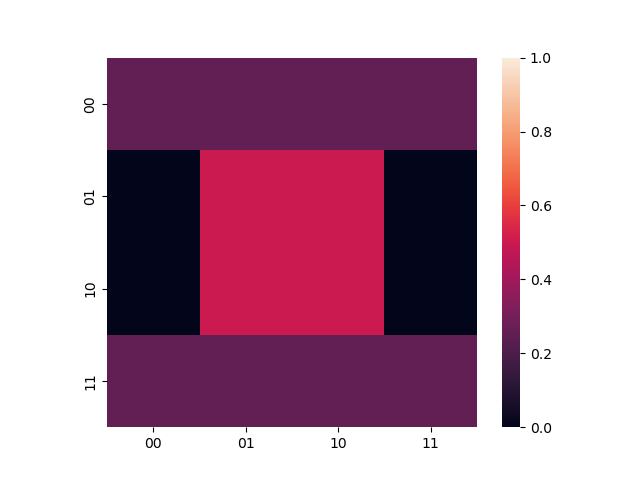
\includegraphics[height=2in]{../plots/very_uneven_prior_editor_init.png}
\end{subfigure}
\begin{subfigure}[t]{0.45\textwidth}
\centering
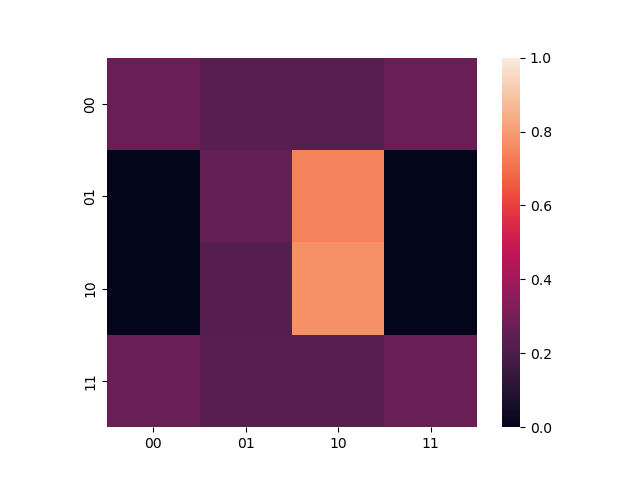
\includegraphics[height=2in]{../plots/very_uneven_prior_editor_final.png}
\end{subfigure}
\caption{
\label{fig:editor-toy}
The emission probabilities for the editor model at the start of training (left)
and end of training (right).
}
\end{figure}

\begin{figure}[h]
\centering
\begin{subfigure}[t]{0.45\textwidth}
\centering
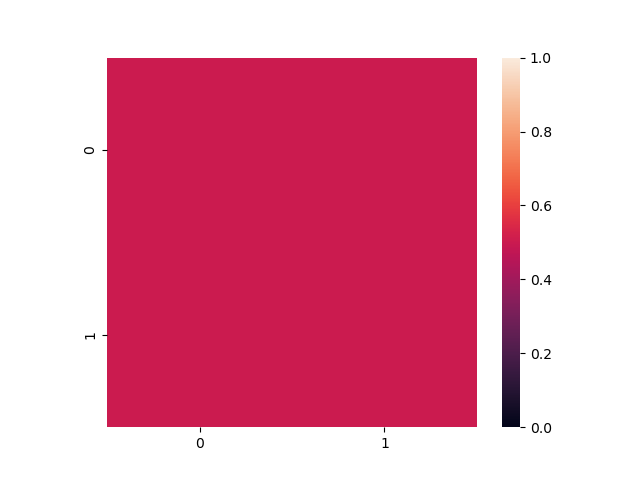
\includegraphics[height=2in]{../plots/very_uneven_prior_student_init.png}
\end{subfigure}
\begin{subfigure}[t]{0.45\textwidth}
\centering
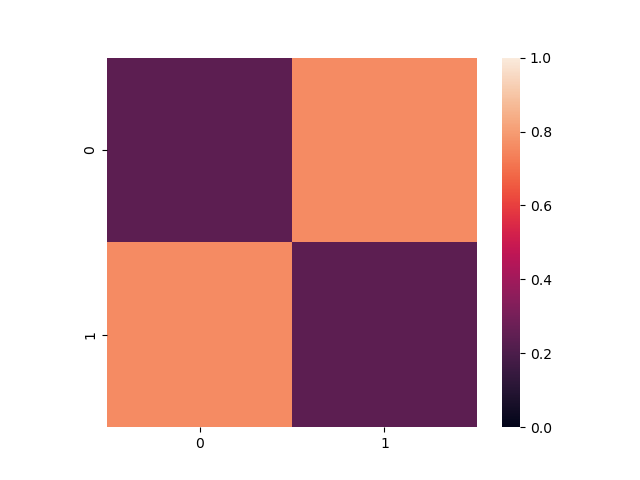
\includegraphics[height=2in]{../plots/very_uneven_prior_student_final.png}
\end{subfigure}
\caption{
\label{fig:student-toy}
The emission probabilities for the student model at the start of training (left)
and end of training (right).
}
\end{figure}

However, in settings where the true data distribution is less skewed,
the objective does not allow the edit model to deviate too far.
Figures \ref{fig:editor-toy2} and \ref{fig:student-toy2} show the results
when $b = [1e-3, 0.5, 0.5, 1-e3]$.
In this setting, both the data distribution and edit distribution are symmetric,
resulting in the student remaining at a standstill.
This is because any movement away from the true distribution would incur
too large a penalty in the first term of the objective,
$\KL{p(y) || \sum_y q(\hat{y} \mid y)p(y)}$.

\begin{figure}[h]
\centering
\begin{subfigure}[t]{0.45\textwidth}
\centering
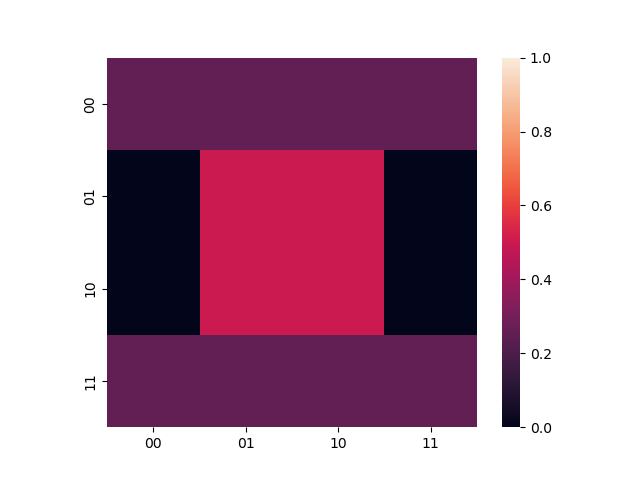
\includegraphics[height=2in]{../plots/even_prior_editor_init.png}
\end{subfigure}
\begin{subfigure}[t]{0.45\textwidth}
\centering
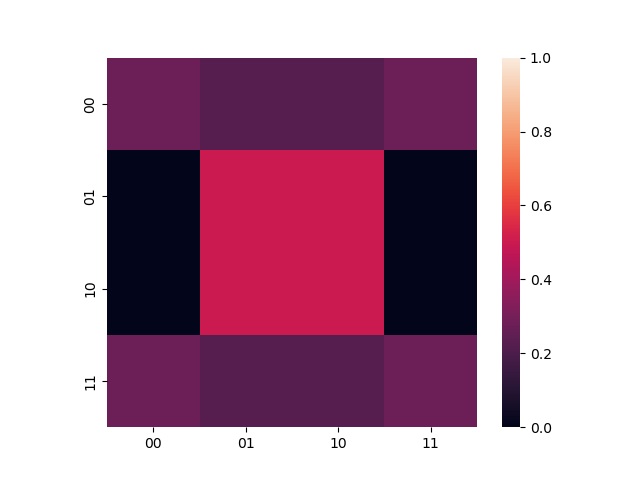
\includegraphics[height=2in]{../plots/even_prior_editor_final.png}
\end{subfigure}
\caption{
\label{fig:editor-toy2}
The emission probabilities for the editor model at the start of training (left)
and end of training (right) with an even true data distribution.
}
\end{figure}

\begin{figure}[h]
\centering
\begin{subfigure}[t]{0.45\textwidth}
\centering
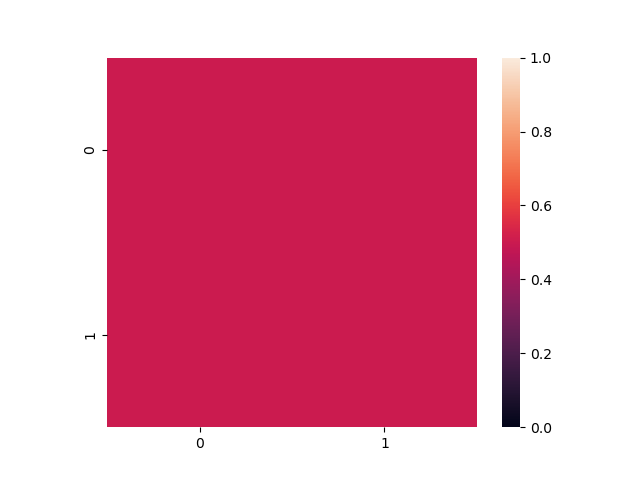
\includegraphics[height=2in]{../plots/even_prior_student_init.png}
\end{subfigure}
\begin{subfigure}[t]{0.45\textwidth}
\centering
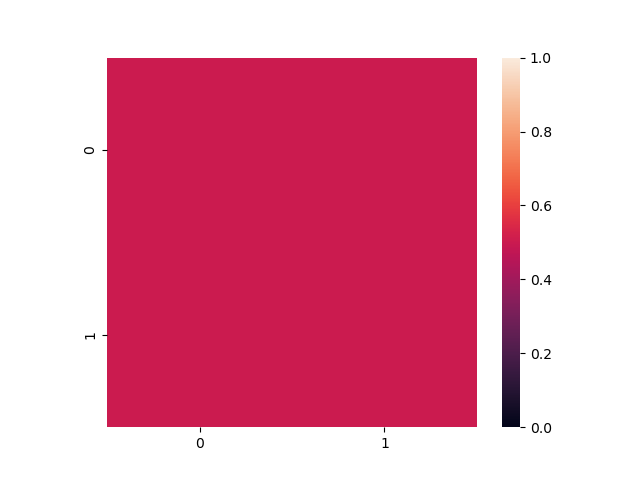
\includegraphics[height=2in]{../plots/even_prior_student_final.png}
\end{subfigure}
\caption{
\label{fig:student-toy2}
The emission probabilities for the student model at the start of training (left)
and end of training (right) with an even true data distribution.
}
\end{figure}


\bibliography{bib}

\end{document}
